\documentclass[tikz,border=3pt]{standalone}
\usepackage[utf8]{inputenc}
\usepackage[T1]{fontenc}
\usepackage{lmodern}
\renewcommand{\familydefault}{\sfdefault}
\usepackage{sansmath}\sansmath
\usepackage{chemfig}
\usepackage{pgfplots}\pgfplotsset{compat=1.18,/pgf/number format/use comma,/pgf/number format/1000 sep={.}}
\usetikzlibrary{arrows.meta,calc,positioning,decorations.pathmorphing,patterns}
% paleta del sitio
\definecolor{nar}{HTML}{E8680C}\definecolor{narc}{HTML}{FFB35C}\definecolor{hielo}{HTML}{FFF3E8}
\definecolor{tinta}{HTML}{1D1D1F}\definecolor{gris}{HTML}{6E6E73}\definecolor{lila}{HTML}{7C5CF0}
\definecolor{azul}{HTML}{2F6FD6}\definecolor{menta}{HTML}{17A673}\definecolor{coral}{HTML}{E8342A}
\begin{document}
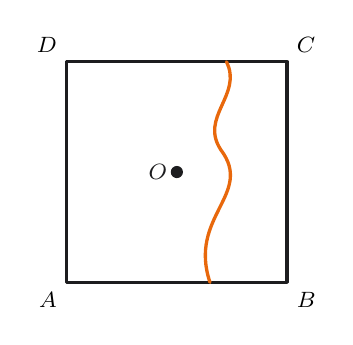
\begin{tikzpicture}[font=\small,x=0.7cm,y=0.7cm,line cap=round,line join=round,step={(1,1)}]
\draw[tinta,very thick] (0,0) rectangle (4,4);
\draw[nar,very thick] (2.6,0) .. controls (2.2,1.2) and (3.4,1.6) .. (2.8,2.4) .. controls (2.4,3.0) and (3.2,3.4) .. (2.9,4);
\fill[tinta] (2,2) circle (2.2pt) node[left,font=\footnotesize] {$O$};
\node[below left,font=\footnotesize] at (0,0) {$A$}; \node[below right,font=\footnotesize] at (4,0) {$B$};
\node[above right,font=\footnotesize] at (4,4) {$C$}; \node[above left,font=\footnotesize] at (0,4) {$D$};
\end{tikzpicture}
\end{document}
